\section{Alert generati}

Esponiamo per una più chiara interpretazione del grafico a seguito di che genere di eventi gli alert vengono generati:

\begin{itemize}

    \item \textbf{ICMP PING undefined code}, questo alert vine generato quando un utente esterno effettua un ping su un server interno usando una richiesta di tipo echo ICMP. Generalmente un attaccante utilizza scansioni di questo tipo per ottenere informazioni sul network o inviare un elevato numero di ping nel tentativo di causare un flood della rete per creare un DoS.

    \item \textbf{ICMP Echo Reply undefined code}, questo alert viene generato quando un host genera una risposta di tipo echo ICMP, (con un codice ICMP non valido o non denito). \'E evidente che questo messaggio è speculare rispetto al precedente: l'host di destinazione invia un messaggio di risposta all'host richiedente indicando quindi di essere alive.

    \item \textbf{SNMP AgentX/tcp request}, questo alert viene generato quando si tenta di attaccare un dispositivo utilizzando SNMP v1. L'impatto varia in base all'implementazione, da un tentativo di Denial of Service (DoS) all'esecuzione di codice. SNMP (Simple Network Management Protocol) è un protocollo largamente adottato per reti IP, utile ai ni di manutenzione e monitoring.

    \item \textbf{SNMP request tcp}, questo alert viene generato quando si invia una richiesta per determinare se un dispositivo stia usando l'SNMP; l'attaccante invia un pacchetto (solitamente diretto alla porta tcp o udp 161), e se ciò avviene con successo viene generata una risposta, in base alla quale potrà scegliere di inviare eventuali ulteriori attacchi all'SNMP daemon.

    \item \textbf{SHELLCODE x86 inc ebx NOOP}, questo alert viene generato quando è probabile sia stato effettuato un tentativo di eseguire del codice su di un host nella rete protette proveniente da una sorgente esterna a tale rete.

    \item \textbf{SCAN nmap XMAS}, questo alert viene generato quando è stata individuata una scansione da parte della piattaforma XMAS di Nmap.Generalmente avviene quando un attaccante effettua una scansione con Nmap al fine di determinare quali siano le porte aperte, esattamente ciò che abbiamo effettuato. Ciò significa che SNORT ha individuato la nostra scansione con Nmap.

    \item \textbf{ICMP PING}, questo alert viene generato quando viene effettuata una richiesta ICMP echo di tipo generico per determinare se l'host è attivo. Analogo all'ICMP PING undefined code.
        
    \item \textbf{ICMP Echo Reply}, analogo all'ICMP PING Echo Reply undefined code.
    
    \item \textbf{ICMP Destination Unreachable Port Unreachable}, questo alert può indicare che che qualcuno ha tentato di connettersi ad una porta o ad un sistema non disponibile e che probabilmente la sorgente di un determinato pacchetto sta effettuando una scansione o un'altra attività maligna.
        
    \item \textbf{ICMP PING *NIX}, questo alert indica che è stato effettuato un ping originato da un host su cui è in esecuzione Unix.
        
    \item \textbf{SNMP public access udp}, questo alert viene generato quando si effettua una connessione di tipo SNMP tramite UDP utilizzando la community 'public'; molte implementazioni di SNMP sono preconfigurate con communities 'public' e 'private' e se non vengono disabilitate un attaccante può tentare di ottenere informazioni sul dispositivo.
        
    \item \textbf{SNMP request udp},è un alert analogo all'SNMP request tcp,generato quando si invia una richiesta per determinare se un dispositivo stia usando l'SNMP; in questo caso la porta sulla quale l'attaccante invia un pacchetto è di tipo udp.
        
    \item \textbf{MS-SQL ping attempt}, questo alert viene generato quando si identifica un tentativo di SQL ping nel traffico di rete. SNORT segnala che può essere stato utilizzato Nessus per accertarsi dell'esistenza di un database SQL sull'host e può preludere ad un attacco verso tale servizio o indicare che altri tool siano in uso per determinare lo stato dei server SQL.
        
    \item \textbf{POLICY PCAnywhere server response}, questo alert viene generato quando il traffico di rete indica l'utilizzo di un'applicazione o di un servizio potenzialmente in grado di violare una politica di corporate security. Una violazione della politica di corporate security può manifestare un serio rischio per le attività della compagnia.
        
    \item \textbf{RPC portmap listing UDP 111}, il servizio di mappatura delle porte registra tutti i servizi RPC (Remote Procedure Call) sugli host di tipo UNIX. Quando un evento generato quando è possibile che sia stato effettuato un tentativo di scoprire quali servizi RPC siano offerti e su quali porte siano in ascolto.
        
    \item \textbf{DNS named version attempt}, questo alert viene generato quando viene effettuato un tentativo di scoprire la versione di BIND (Berkeley Internet Name Domain, il più usato specialmente su sistemi Unix) specifica che il server DNS sta eseguendo. Così facendo un potenziale attaccante può scoprire quali server siano potenzialmente vulnerabili a degli exploit associati ad una versione di BIND.
        
    \item \textbf{ICMP traceroute}, questo alert viene generato quando è probabile sia stato identificato Windows traceroute, comando generalmente utilizzato da un attaccante che voglia determinare gli host ed i router attivi su una rete in preparazione di un attacco.
        
    \item \textbf{SNMP missing community string attempt}, questo alert viene generato quando le comunicazioni SNMP non contengono un nome di community. Un nome di community SNMP è il processo di autenticazione che un host, che esegue SNMP, utilizza per concedere l'accesso. Fornendo una community vuota e un attaccante può tentare di ottenere l'accesso a funzionalità SNMP per un dispositivo che non è correttamente ben configurato.
        
    \item \textbf{ICMP PING BSDtype}, questo alert indica che è stata inviata dalla rete una richiesta di ping Questo genere di richieste solitamente vengono utilizzate per determinare se un host è "reponsive", ma sono anche  utilizzabili per mappare la rete.
    
    \item \textbf{TOO MUCH PING}, questo alert viene generato ogni qualvolta che il numero di ping sottomessi al secondo sono più di 10. Permette di rilevare una sorta di DoS improntato su un eccessivo invio di ping verso l'host monitorato.
    
    \item \textbf{SNMP private access udp}, questo alert viene generato quando viene stabilita una connessione SNMP su UDP utilizzando la community di default. SNMP (Simple Network Management Protocol) utilizza le community e gli indirizzi IP per autenticare la comunicazione tra il client SNMP e il demone SNMP. Molte implementazioni di SNMP sono preconfigurate con community "private" e "public". Se queste non sono disattivati, l'attaccante può raccogliere una grande quantità di informazioni sul dispositivo che esegue il demone SNMP.

\end{itemize}

Analizzando i tempi di detection raggruppati e mediati per tipo di alert generato, vediamo come ci siano due tipi di alert, "SNMP request tcp" e "SNMP AgentX/tcp request" (per comodità visualizzati a parte), che registrano dei tempi di rilevazione molto più alti della media: gli attacchi che generano questi alert (metasploit ed nmap) sono tra i più difficili da rilevare tra quelli esaminati in questi esperimenti. Osservando i valori di detection relativi agli altri alert, possiamo vedere come in generale gli alert di pacchetti ICMP siano quelli più velocemente rilevati (alcuni di essi hanno addirittura tempo di rilevazione nullo rispetto all'arrivo del primo pacchetto), mentre altri, come ad esempio "SCAN nmap XMAS", richiedano più tempo per essere rilevati da Snort.\\
Inoltre analizzando il tempo di detection per ogni singolo alert generato si può vedere che attacchi più specifici del semplice ping sul protocollo ICMP hanno un tempo di detection più alto. Come ad esempio \textit{ICMP PING undefined code} e \textit{ICMP Echo Reply undefined code}.

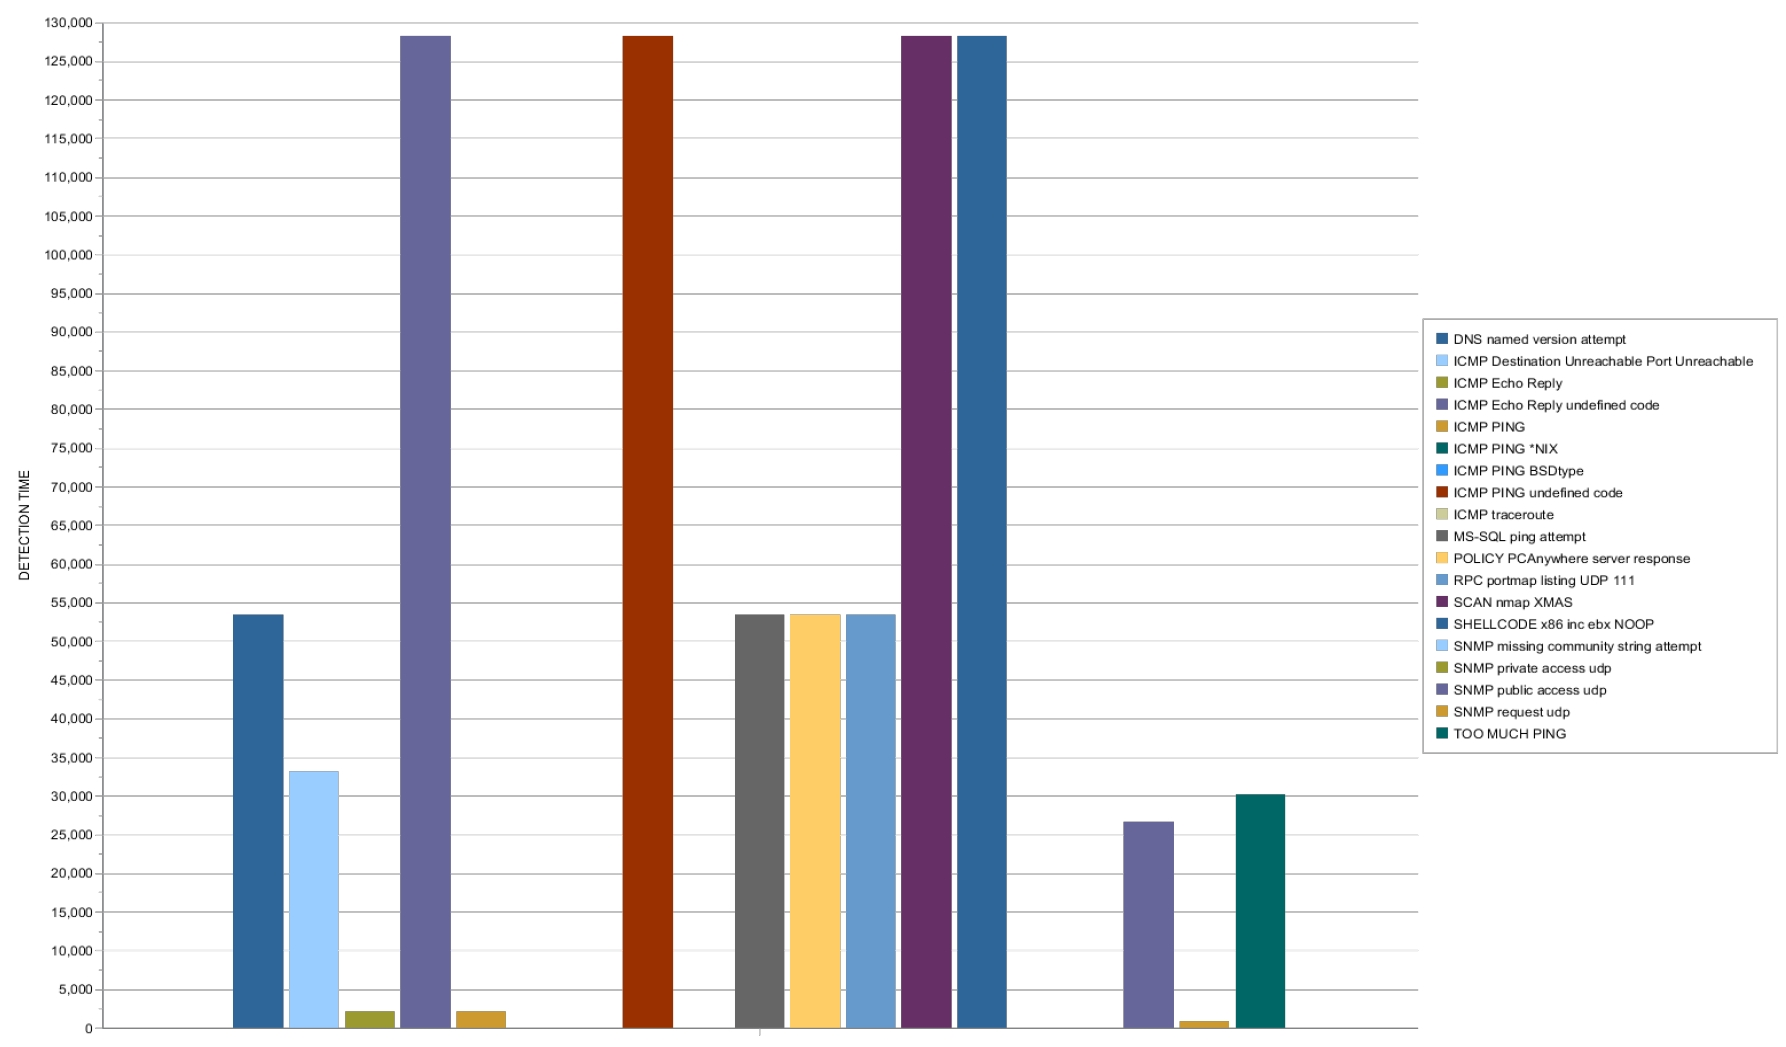
\includegraphics[scale=0.3]{figure/detection_msg.jpg}\\

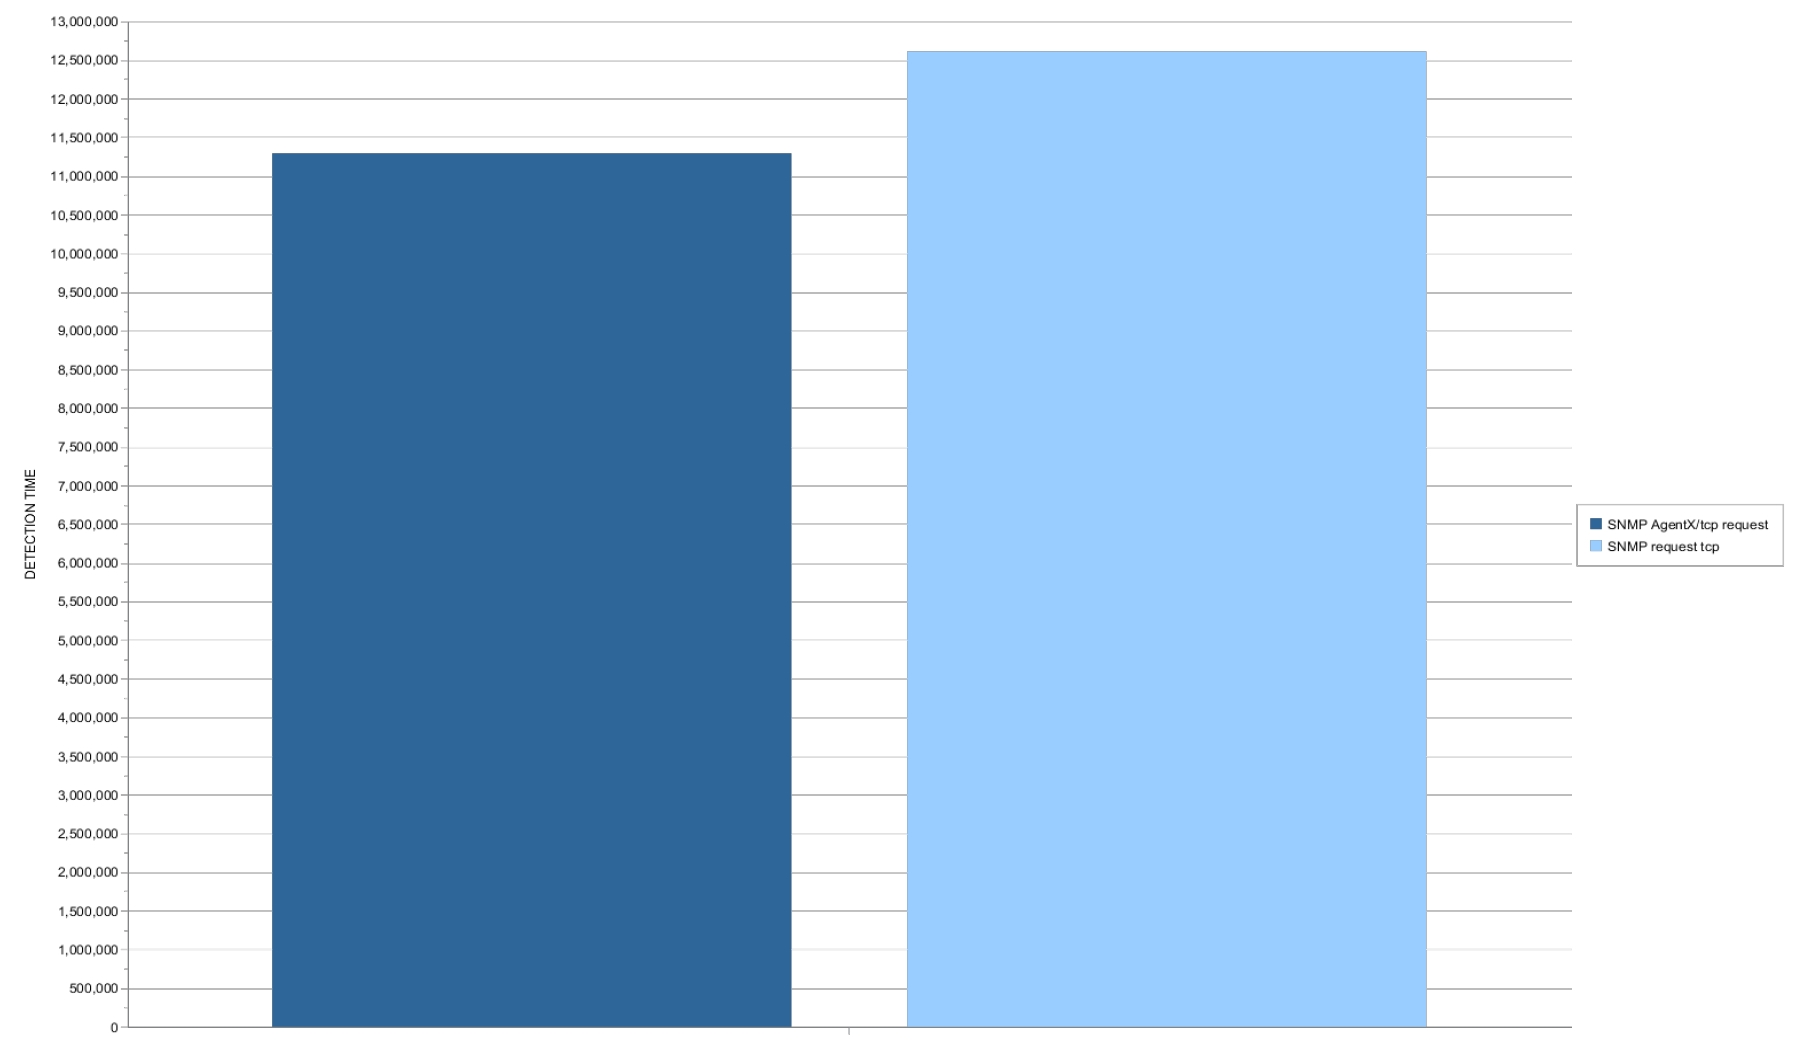
\includegraphics[scale=0.3]{figure/detection_SNMP.jpg}\\

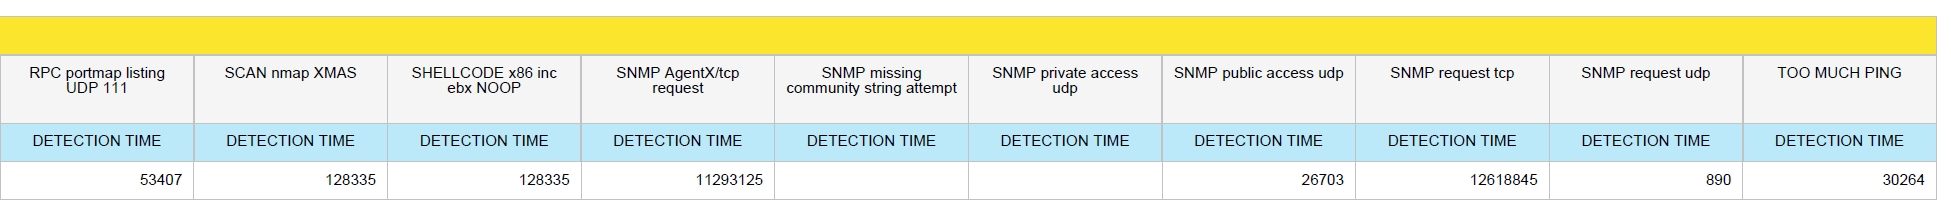
\includegraphics[scale=0.25]{figure/tabella_detection_msg_2.jpg}\\

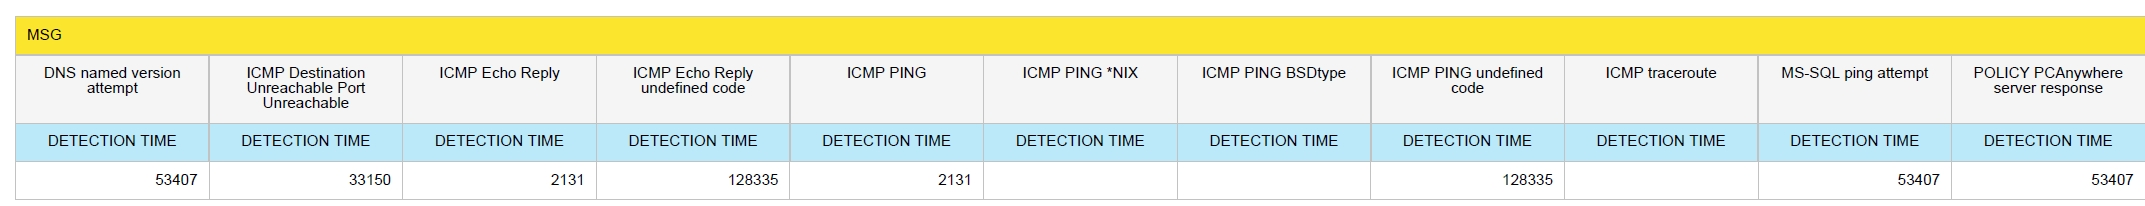
\includegraphics[scale=0.25]{figure/tabella_detection_msg_1.jpg}
